\documentclass[journal]{IEEEtran}
\usepackage[a5paper, margin=10mm, onecolumn]{geometry}
\usepackage[cmex10]{amsmath}
\usepackage{amssymb,amsfonts,amsthm}
\usepackage{gvv-book}
\usepackage{gvv}
\usepackage{hyperref}
\usepackage{physics}
\usepackage{gauss}

\begin{document}
\title{4.13.30}
\author{EE25BTECH11025 - Ganachari Vishwambhar}
\maketitle

\textbf{Question}:\\
If $\vec{P}=(1,0)$, $\vec{Q} = (-1,0)$  and $\vec{R}=(2,0)$ are three given points, then the locus of point $\vec{S}$ satisfying the relation $(SQ)^2+(SR)^2=2(SP)^2$, is:\\
\begin{enumerate}
    \item a straight line parallel to $X$ axis
    \item a circle passing through the origin
    \item a circle with the center at the origin
    \item a straight line parallel to $Y$ axis
\end{enumerate}
\textbf{Solution: }\\
Given:
\begin{align}
    \vec{P}=\myvec{1\\0}; \vec{Q}=\myvec{-1\\0}; \vec{R}=\myvec{2\\0}\\
    \vec{S}=\myvec{x\\y}
\end{align}

Solving:
\begin{align}
    ||\vec{Q}-\vec{S}||^2+||\vec{R}-\vec{S}||^2=2||\vec{P}-\vec{S}||^2\\
    \myvec{\vec{Q}-\vec{S}}^\top\myvec{\vec{Q}-\vec{S}}+\myvec{\vec{R}-\vec{S}}^\top\myvec{\vec{R}-\vec{S}}=2\myvec{\vec{P}-\vec{S}}^\top\myvec{\vec{P}-\vec{S}}\\
    ||\vec{Q}||^2+||\vec{R}||^2-2||\vec{P}||^2=\vec{S}^\top+\vec{Q}^\top\vec{S}+\vec{S}^\top\vec{R}+\vec{R}^\top\vec{S}-2\vec{S}^\top\vec{P}-2\vec{P}^\top\vec{S}\\
    ||\vec{Q}||^2+||\vec{R}||^2-2||\vec{P}||^2=\vec{S}^\top\myvec{\vec{Q}+\vec{R}-2\vec{P}}+\vec{S}\myvec{\vec{Q}+\vec{R}-2\vec{P}}^\top\\
    ||\vec{Q}||^2+||\vec{R}||^2-2||\vec{P}||^2=2\myvec{\vec{Q}+\vec{R}-2\vec{P}}^\top\vec{S}
\end{align}

Equation (7) is of the form:
\begin{align}
    \vec{n}^\top\vec{x}=c\\
    \myvec{\vec{Q}+\vec{R}-2\vec{P}}^\top\vec{S}=\frac{||\vec{Q}||^2+||\vec{R}||^2-2||\vec{P}||^2}{2}
\end{align}

Substituting values:
\begin{align}
    \myvec{\myvec{-1\\0}+\myvec{2\\0}-2\myvec{1\\0}}^\top\vec{S}=\frac{\brak{\brak{-1}^2+0^2}+\brak{2^2+0^2}-2\brak{1^2+0^2}}{2}\\
    \myvec{-1\\0}^\top\vec{S}=\frac{3}{2}
\end{align}

Hence the locus of $\vec{s}$ is a line parallel to $Y$-axis.

\begin{figure}[h!]
   \centering
   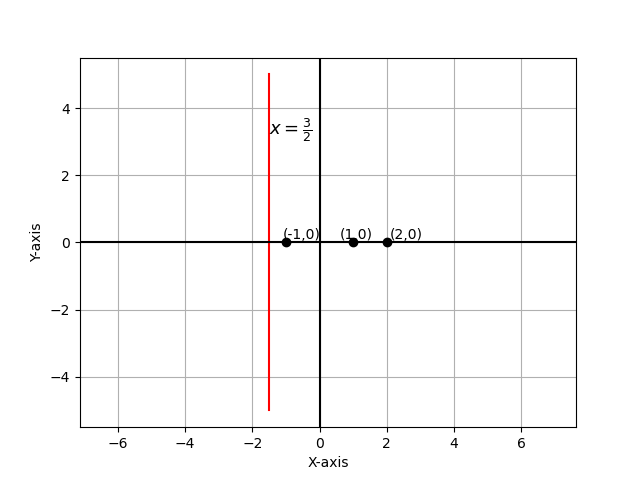
\includegraphics[width=0.7\linewidth]{figs/plot.png}
   \caption{Plot of the given points and locus of $\vec{S}$}
   \label{}
\end{figure}
\end{document}  